%%%%%%%%%%%%%%%%%%%%%%%%%%%%%%%%%%%%%%%%%%%%%%%%%%%%%%%%%%%%%%%%%%%%%%%
%%%%  Load the document class and packages                         %%%%
%%%%%%%%%%%%%%%%%%%%%%%%%%%%%%%%%%%%%%%%%%%%%%%%%%%%%%%%%%%%%%%%%%%%%%%
\documentclass[a4paper]{report}
\usepackage{epsfig}            % to insert PostScript figures
\graphicspath{ 
	{./figures/} 
}

%Change figure names
\renewcommand{\figurename}{Fig}

\usepackage[bf,footnotesize]{caption} % make captions small and label bold

\addtocounter{chapter}{1} %Because starting at zero is silly
\makeatletter
\renewcommand{\thesection}{\@arabic\c@section}
\renewcommand{\thefigure}{\@arabic\c@figure}
\makeatother

\usepackage{titlesec} %change spacing before and after sections
%format: \titlespacing*{<command>}{<left>}{<before-sep>}{<after-sep>}
\titlespacing*{\section}{0pt}{11mm plus 1ex minus .2ex}{6mm plus .2ex}
\titlespacing*{\subsection}{0pt}{9mm plus 1ex minus .2ex}{4mm plus .2ex}

\usepackage[a4paper,margin=3.7cm,tmargin=2.5cm,bmargin=2.5cm]{geometry} 
\usepackage{textcomp}          % To make nice degree symbols and others\usepackage[bf,footnotesize]{caption} % make captions small and label bold
\usepackage{wrapfig}
%to produce the clickable references along the left in Acroread. This
%package must be included last. 
\usepackage[ps2pdf,bookmarks=TRUE]{hyperref} 
\hypersetup{
    colorlinks=true,
    linkcolor=cyan,
    filecolor=magenta,      
    urlcolor=cyan,
}

%%%%%%%%%%%%%%%%%%%%%%%%%%%%%%%%%%%%%%%%%%%%%%%%%%%%%%%%%%%%%%%%%%%%%%%
%%%%  Hypertext references for Acrobat                             %%%%
%%%%%%%%%%%%%%%%%%%%%%%%%%%%%%%%%%%%%%%%%%%%%%%%%%%%%%%%%%%%%%%%%%%%%%%
\hypersetup{
	pdfauthor = {SWC},
	pdftitle = {Optics Exercises},
	pdfkeywords = {optics, lenses, refraction, reflection, dispersion,
		telescope, microscope},
	pdfcreator = {LaTeX with hyperref},
	pdfproducer = {dvips + ps2pdf}
}

%%%%%%%%%%%%%%%%%%%%%%%%%%%%%%%%%%%%%%%%%%%%%%%%%%%%%%%%%%%%%%%%%%%%%%%
%%%%  Main text                                                    %%%%
%%%%%%%%%%%%%%%%%%%%%%%%%%%%%%%%%%%%%%%%%%%%%%%%%%%%%%%%%%%%%%%%%%%%%%%
\begin{document}
	
	%set the number of sectioning levels 
	\setcounter{secnumdepth}{2}
	
	\begin{center}
		\textbf{\Large{Building an epifluorescence microscope}}
	\end{center}
	
	%%%%%%%%%%%%%%%%%%%%%%%%%%%%%%%%%%%%%%%%%%%%%%%%%%%%%%%%%%%%%%%%%%%%%%%
%	\section{Introduction}
	%%%%%%%%%%%%%%%%%%%%%%%%%%%%%%%%%%%%%%%%%%%%%%%%%%%%%%%%%%%%%%%%%%%%%%%
	\vspace{0.8cm}
	\noindent The goal of this series of exercises is to build a standard epi-fluorescence microscope. At the end, you will take wonderful pictures of auto-fluorescent and GFP-labeled samples.
	
%    \begin{itemize}
%	    \item Bullet points are things to do
%	    \item Hints are at the end of the document. Click on `Go to hint' and `Go back' to navigate. Don't just read the hint right away, but be sure to read it before moving on.
%	    \item Help with the assembly of optics parts can be found in `Assembly Instructions'.
%	\end{itemize}
	\\
	\\
%	\textbf{current ToDos:} \\
%	- put pictures of setup \\


    %%%%%%%%%%%%%%%%%%%%%%%%%%%%%%%%%%%%%%%%%%%%%%%%%%%%%%%%%%%%%%%%%%%%%%%
	\section{Illuminating the sample}
	%%%%%%%%%%%%%%%%%%%%%%%%%%%%%%%%%%%%%%%%%%%%%%%%%%%%%%%%%%%%%%%%%%%%%%%
	\hypertarget{hintBack-illumination}{}
	A feature of the fluorescence process is that it is \emph{isotropic}: the emitted light is independent of the excitation light (in terms of direction). 
	\begin{itemize}
	    \item What are the important points about how to illuminate the sample for an epi-fluorescence microscope?
    \end{itemize}
    
    Fluorescence microscopy only works thanks to the Stokes shift: the emission photons can be separated from the excitation photons. This provides images with great contrast, \emph{provided the excitation light is blocked out well enough}.
    \begin{itemize}
	    \item What filters do you need and where should they be placed?
	    \item Draw the ray diagram of your illumination pathway and build it. \textbf{Coarse alignment:} Take care to put all optical elements at the same height. In particular, the blue illumination light should exit the objective straight (not traveling up/down/sideways).
	\end{itemize}
	
	\hyperlink{hintTo-illumination}{Go to hint}
	\\
	
	
	%%%%%%%%%%%%%%%%%%%%%%%%%%%%%%%%%%%%%%%%%%%%%%%%%%%%%%%%%%%%%%%%%%%%%%%
	\section{Imaging the sample}
	%%%%%%%%%%%%%%%%%%%%%%%%%%%%%%%%%%%%%%%%%%%%%%%%%%%%%%%%%%%%%%%%%%%%%%%
	Let's set up the imaging optics and camera.
    \begin{itemize}
        \item \textbf{Coarse alignment:} Take care to put all optical elements at the same height, so the objective--cube--tube lens--camera axis is level.
        \item You will be using a 300~mm tube lens that is already mounted in a short SM1 lens tube. 
        \item The images we take will be very sensitive to light pollution -- we get very few (green) photons back. Put SM1 lens tubes on the cube and the camera, then slide on the plastic tube to cover the path in between (keep the tube lens--camera chip distance correct!). Also make sure there is minimal light entering the objective that is not coming from the sample.
        \item Make sure to set the gain and exposure of the camera adequately.
        \item Image a simple sample first, i.e. highlighter on paper. Then test unlabeled tissue paper and finally pollen grain, diatoms and brain slices
        
    \end{itemize}
	\hypertarget{hintBack-imaging}{}
	
    
	\\
	\hyperlink{hintTo-imaging}{Go to hint}
	
	
	%%%%%%%%%%%%%%%%%%%%%%%%%%%%%%%%%%%%%%%%%%%%%%%%%%%%%%%%%%%%%%%%%%%%%%%
	\section{Challenge questions}
	%%%%%%%%%%%%%%%%%%%%%%%%%%%%%%%%%%%%%%%%%%%%%%%%%%%%%%%%%%%%%%%%%%%%%%%
	\hypertarget{hintBack-challenge}{}
	
	%----------------------------------------------------------------------
	\subsection{Blocking the excitation light}
	%----------------------------------------------------------------------
    Filters mainly use interference to manipulate what light passes through. 
    
	\\
	\hyperlink{hintTo-challenge}{Go to hint}
	
	
	\clearpage
    %%%%%%%%%%%%%%%%%%%%%%%%%%%%%%%%%%%%%%%%%%%%%%%%%%%%%%%%%%%%%%%%%%%%%%%
    %%%%%%%%%%%%%%%%%%%%%%%%%%%%%%%%%%%%%%%%%%%%%%%%%%%%%%%%%%%%%%%%%%%%%%%
    %%%%%%%%%%%%%%%%%%%%%%%%%%%%%%%%%%%%%%%%%%%%%%%%%%%%%%%%%%%%%%%%%%%%%%%
    
	%%%%%%%%%%%%%%%%%%%%%%%%%%%%%%%%%%%%%%%%%%%%%%%%%%%%%%%%%%%%%%%%%%%%%%%
	\section{Hints and Help}
	%%%%%%%%%%%%%%%%%%%%%%%%%%%%%%%%%%%%%%%%%%%%%%%%%%%%%%%%%%%%%%%%%%%%%%%
	
	%----------------------------------------------------------------------
    \subsection{Hint - Illumination}
    %----------------------------------------------------------------------
	\hypertarget{hintTo-illumination}{}
	
	\subsubsection{Features of illumination}
	Illuminating the sample on an epi-fluorescence microscope has fewer requirements than for the brightfield microscope. We only need to ensure
	\begin{enumerate}
	    \item Uniform illumination: we want to attribute brightness in the image to the presence of fluorophores, not more or less excitation light.
	    \item Control over the field of illumination: exciting fluorophores outside the field of view of the camera incurs unnecessary photodamage and reduces contrast (emitted photons might scatter in the tissue and enter the objective). 
	    \item Control over the brightness of illumination: we need to make sure the sample is only illuminated as minimally as necessary, again to avoid photodamage. In our case, we will limit the current the LED can draw. In other systems, you might want to place an iris in a conjugate plane of the back focal plane of the objective.
	\end{enumerate}
	
	\begin{figure}[h]
		\center
		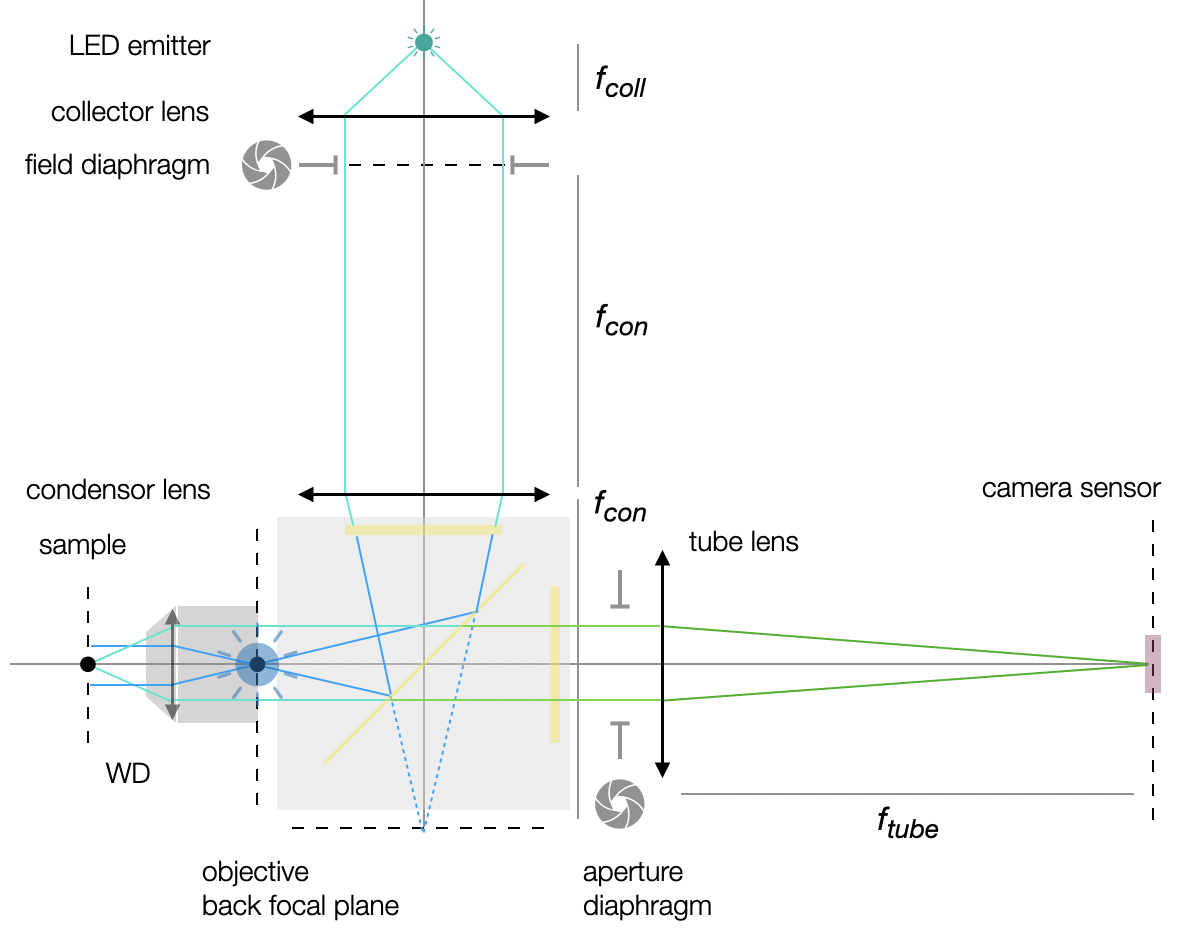
\includegraphics[width=0.9\textwidth]{figures/epifluo.png}
		\captionsetup{width=0.9\textwidth}
		\caption{Epi-fluorescence microscope (seen from above). 
		\\
		Rays are drawn roughly in the correct color: turquoise light from the `blue' LED (it has a broad spectrum, reaching into the green) passes through the excitation filter, reflects off the dichroic mirror, and hits the sample in blue; green light emitted by GFP passes through the dichroic and emission filter.}
		\label{fig:epifluo}
	\end{figure}
	
	
	
	    
	\\
    \hyperlink{hintBack-illumination}{Go back}
    
    \clearpage
    
    %----------------------------------------------------------------------
    \subsection{Hint - imaging the sample}
    %----------------------------------------------------------------------
	\hypertarget{hintTo-imaging}{}
	
	
    \\
    \hyperlink{hintBack-imaging}{Go back}
    
    \clearpage
    
    
    \end{document}